\documentclass[tikz,border=5pt]{standalone}
\usepackage{luatexja}
\usepackage[hiragino-pron]{luatexja-preset}
\usepackage{amsmath,amssymb}
\usetikzlibrary{arrows.meta,patterns}

\begin{document}
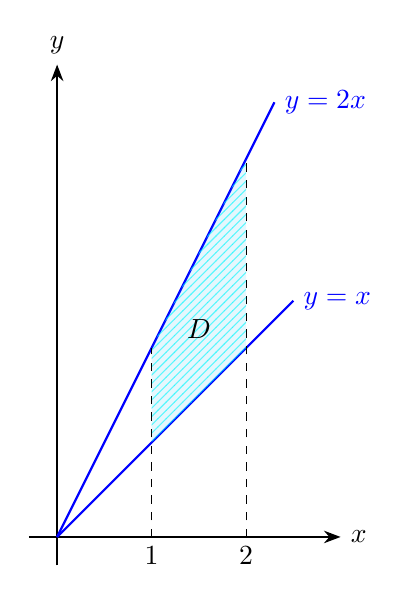
\begin{tikzpicture}[scale=1.2]

% Axes
\draw[-{Stealth[length=6pt]}, thick] (-0.3,0) -- (3,0) node[right] {$x$};
\draw[-{Stealth[length=6pt]}, thick] (0,-0.3) -- (0,5) node[above] {$y$};

% Lines y=x and y=2x
\draw[thick, blue, domain=0:2.5, samples=2] plot (\x, \x) node[right] {$y = x$};
\draw[thick, blue, domain=0:2.3, samples=2] plot (\x, {2*\x}) node[right] {$y = 2x$};

% Fill region D
\fill[pattern=north east lines, pattern color=cyan, opacity=0.6]
  (1,1) -- (2,2) -- (2,4) -- (1,2) -- cycle;
\fill[cyan, opacity=0.1]
  (1,1) -- (2,2) -- (2,4) -- (1,2) -- cycle;

% Boundary lines x=1, x=2
\draw[dashed, thin] (1,0) -- (1,2);
\draw[dashed, thin] (2,0) -- (2,4);

% Labels
\node[below] at (1,0) {$1$};
\node[below] at (2,0) {$2$};
\node at (1.5,2.2) {$D$};

\end{tikzpicture}
\end{document}
